\documentclass{article}
\usepackage[utf8]{inputenc}
\usepackage{amsmath}
\usepackage{geometry}
\usepackage[spanish]{babel}
\usepackage{graphicx}
 
\geometry{top=0.5cm}
 
\title{Mecanica Liner en Ansys}
\author{Cruz Acosta Luis Enrique}
\date{\today}
 
 
\begin{document}
 
\maketitle

\tableofcontents

\begin{abstract}
    Este articulo tiene como objetivo recapitular notas e informacion 
    del curso de Ansys Mecanical Linear que esta tomando el autor en la pagina
    GrupoSSC en el semestre 2022-2
\end{abstract}

\newpage

\section{Modulo \#1 - Mesh}

\section{Modulo \#2 - Preprocessing}

\begin{description}
    \item[1. Static Structural: ] Sera el Analisis de vamos a realizar 
    lo celeccionamos desde el ToolBox  
    \begin{figure}[h!]
        \centering
        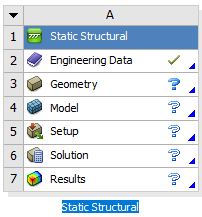
\includegraphics{img/StaticStructural.png}
    \end{figure} 
    
    \item[2. Importar Geometria: ] Aqui es donde le diremos a ANSYS que figura CAD usara 
    para el estudio 

    \begin{figure}[h!]
        \centering
        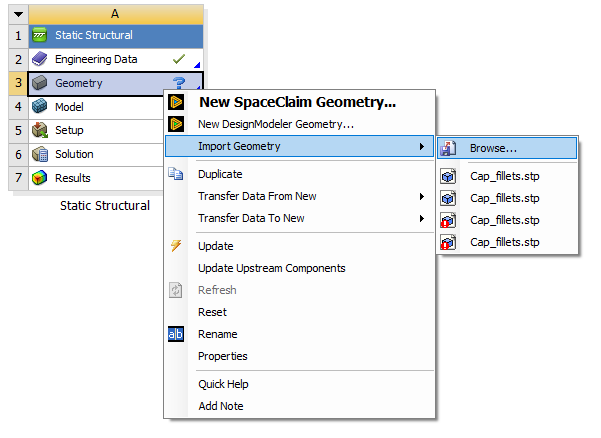
\includegraphics[scale=0.5]{img/importalGeometria.png}
    \end{figure}

    \item[3. Model: ] Es donde aplicaremos todas las condiciones de fronter
    y diremos que estudio estatico se le quiere hacer a nuestra piesa  

    \begin{figure}[h!]
        \centering
        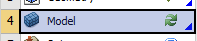
\includegraphics{img/model.png}
    \end{figure}

    Al presionar esa zona, nos abrira la area de "Mecanical" de Ansys 

    \newpage

    \bigskip

    \begin{figure}[h!]
        \centering
        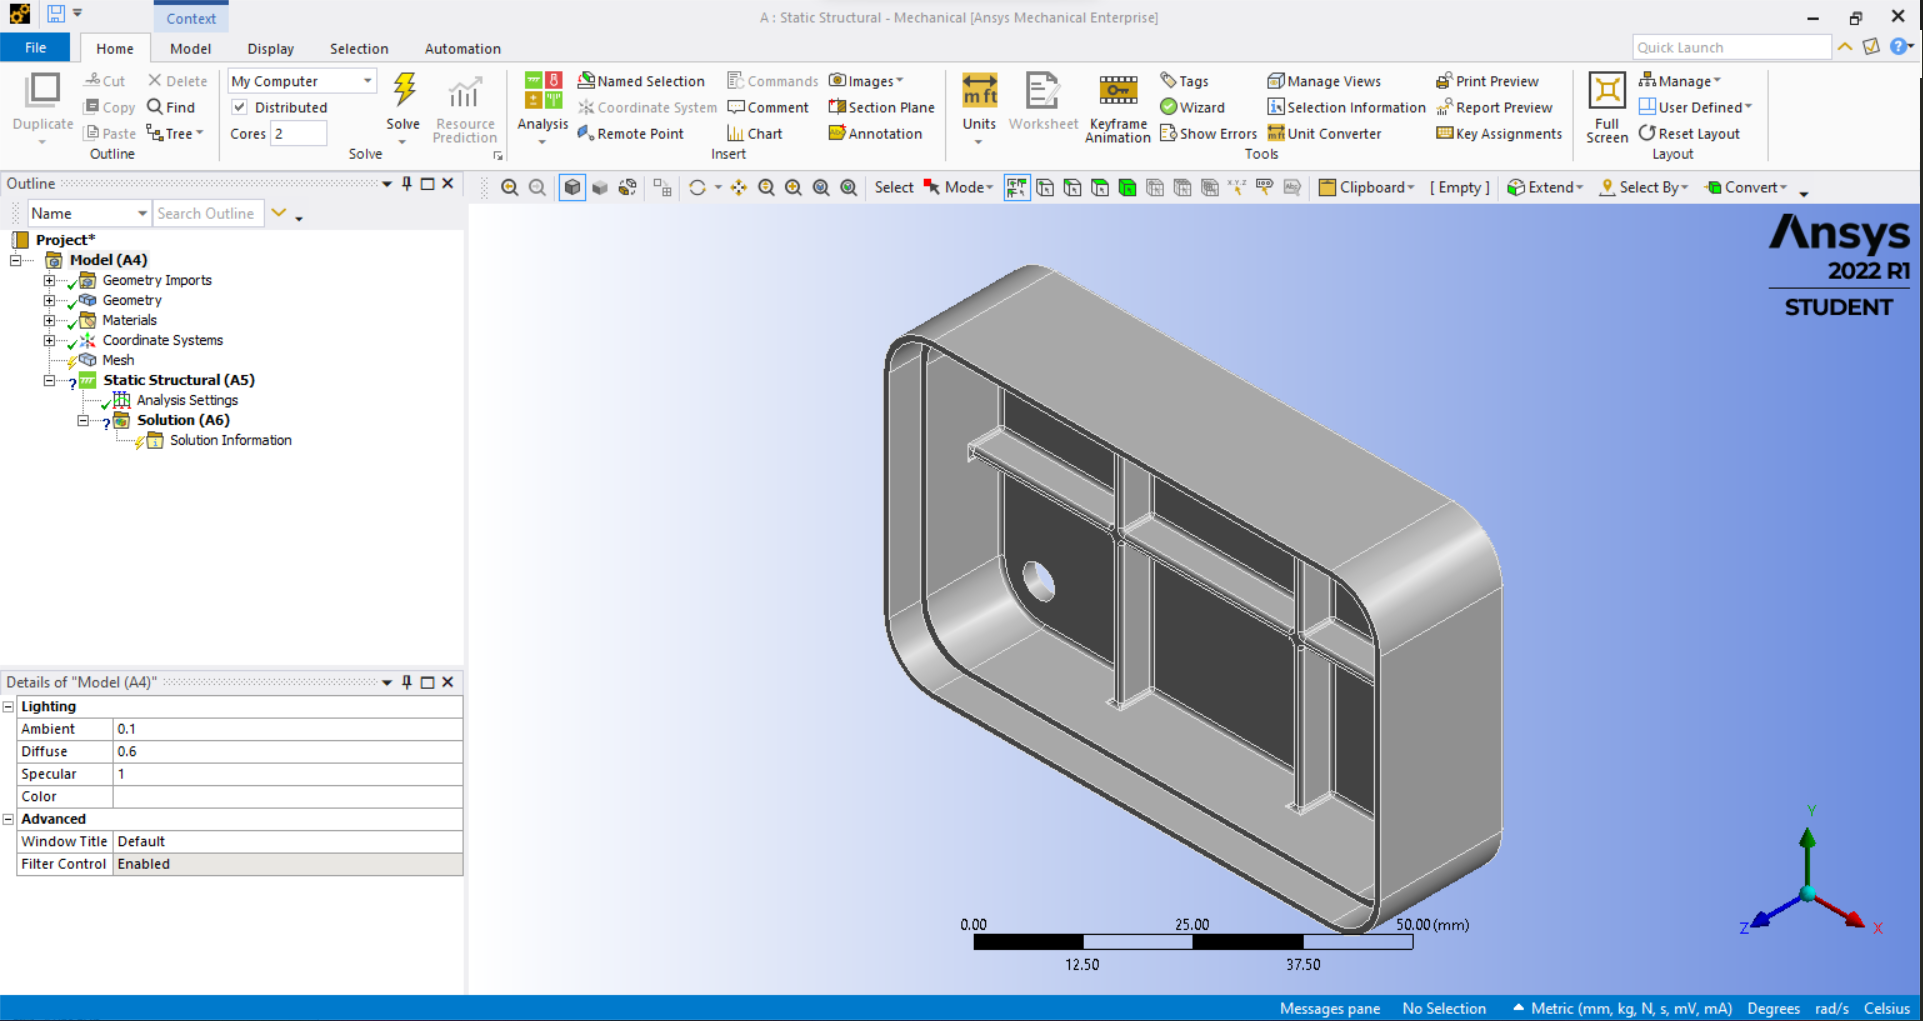
\includegraphics[scale=0.5]{img/mecanical.png}
    \end{figure}

    \begin{description}
        \item[3.1 ] Vamos al arbol del proyecto y cambiamos el material a "Aleacion de aluminio" 
        
        \begin{figure}[h!]
            \centering
            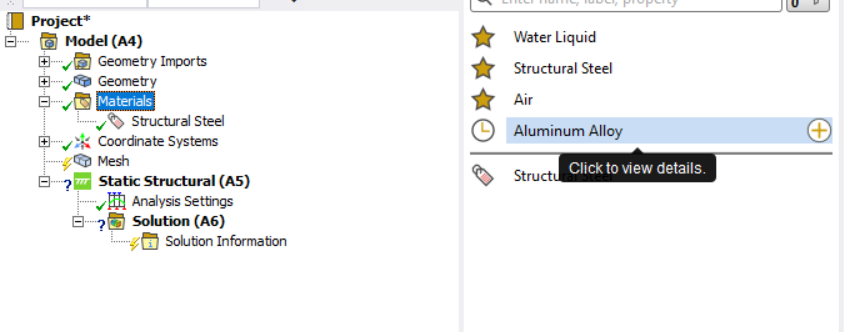
\includegraphics{img/agregarMaterial.png}
        \end{figure}

        \newpage

        \item[3.2 ] Creamos el mesh por defecto 
        \begin{figure}[h!]
            \centering
            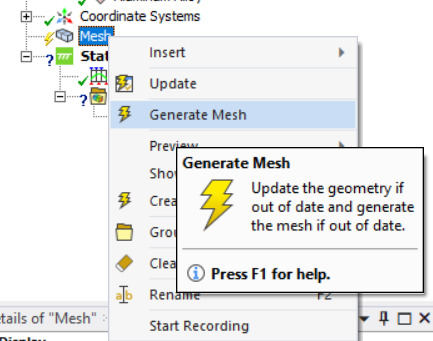
\includegraphics{img/generarMesh.png}
        \end{figure}

        \bigskip

        \begin{figure}[h!]
            \centering
            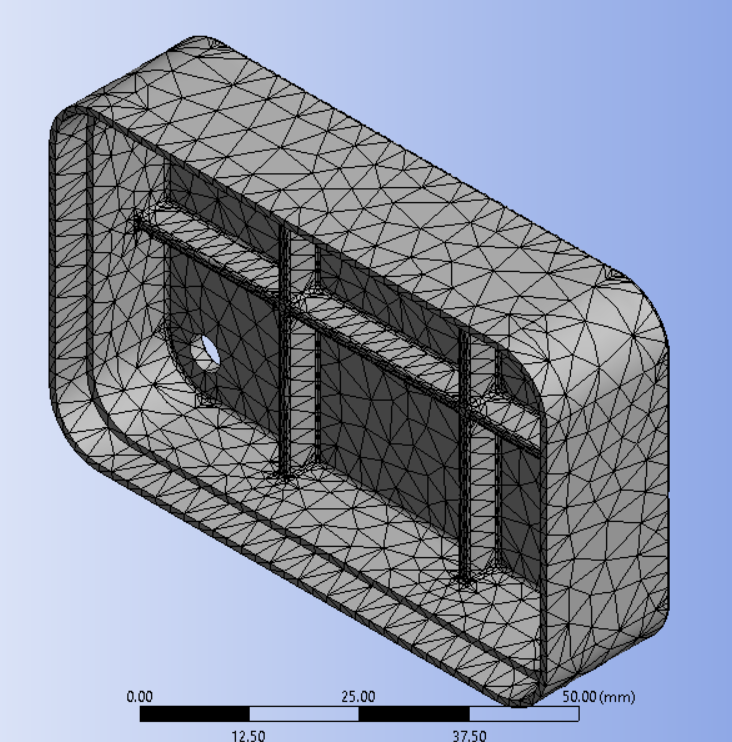
\includegraphics[scale=0.5]{img/malla.png}
        \end{figure}
    \end{description}
\end{description}

 
 
\end{document}